% !TeX program = lualatex
\documentclass[tikz,border=10pt]{standalone}
\usepackage{tkz-graph}
\usepackage{amsmath,amssymb}
\usepackage{xcolor}
\usetikzlibrary{calc}
\usetikzlibrary{positioning, quotes}
\usetikzlibrary{arrows.meta}
\usetikzlibrary{tikzlings}

\tikzset{mytext/.style = {font=\sffamily\bfseries, text=white},
        vertex/.style = {mytext, shape=circle, ball color = #1},
        number/.style = {mytext, draw, fill=red}}

\tikzset{vertex/.default = blue}

\tikzset{highlight/.style = {draw=yellow, very thick, densely dotted},
        highlight vertex/.style = {vertex, highlight},
        highlight number/.style = {number, highlight}}

\tikzset{bridge/.style = {thick ,  double=yellow, double distance= 1pt}}

\begin{document}

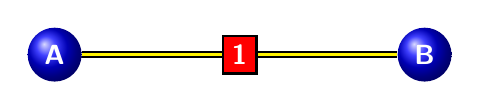
\begin{tikzpicture}
	\node [vertex] (A)  {A};
	\node [vertex, right = 4cm of A] (B)  {B};
	\draw (A) edge[bridge] node[number] {1} (B);
\end{tikzpicture}



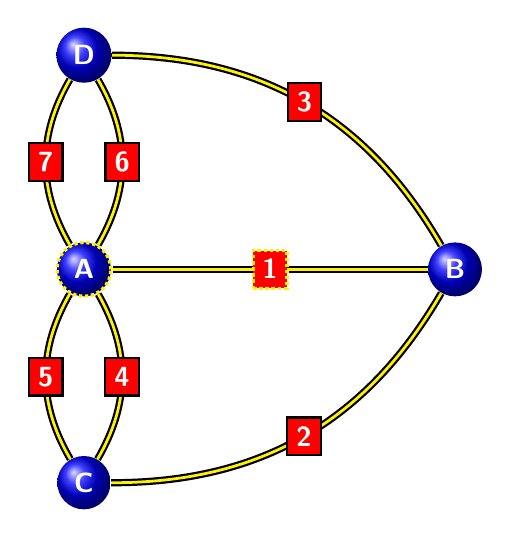
\begin{tikzpicture}
	\node [highlight vertex] (A) {A};
	\node [vertex, right = 4cm of A] (B) {B};
	\draw (A) edge[bridge] node[highlight number] {1}  (B);

	\node [vertex, below=2cm of A] (C)  {C};
	\node [vertex, above=2cm of A] (D) {D};

	\tikzset{bridge/.append style = {bend right}}

	\draw (C) edge [bridge]  node[number] {2} (B)
	(B) edge [bridge] node [number] {3} (D)
	(C) edge [bridge] node [number] {4} (A)
	(A) edge [bridge] node [number] {5} (C)
	(A) edge [bridge] node [number] {6} (D)
	(D) edge [bridge] node [number] {7} (A);
\end{tikzpicture}

\tikzset{smiley/.pic={
			\draw[shading=ball, ball color=yellow] (0,0) circle [radius=2];
			\draw[shading=ball, ball color=black] (-0.5,0.5,0) ellipse [x radius=0.2, y radius=0.4];
			\draw[shading=ball, ball color=black] (0.5,0.5,0) ellipse [x radius=0.2, y radius=0.4];
			\draw[very thick] (-1,-1) arc [start angle=185, end angle=355, x radius=1, y radius=0.5];}}


\begin{tikzpicture}
	\draw pic {smiley}
	(2,2) pic[scale=0.5, rotate=-30] {smiley}
	(-2, 1.5) pic [scale=0.3, rotate=30] {smiley}
	(-1.6, 2) pic [scale=0.15, rotate=-20] {smiley}
	(0, 2) pic [scale= 0.2, rotate=-10] {smiley};
\end{tikzpicture}


\tikzset{mygrid/.pic = {
			\draw[thin, dotted] (-3, -3) grid (3,3);
			\draw [->] (-3, 0) -- (3,0);
			\draw [->] (0, -3) -- (0,3); }}

\begin{tikzpicture}
	\draw pic {mygrid}
	(-1,0)  pic {chicken}
	(1,0)   pic {pig}
	(-2,-2) pic {bear}
	(0,-2)  pic {penguin}
	(2,-2)  pic {owl};
\end{tikzpicture}


\end{document}
